%% generato automaticamente da tools/build_tex.py --- non modificare
\chapter{Un filtro elimina-banda}
\label{cap:notch}
\quaderno{notch.dfw}{21 Jan 2010}{20}

Gennaio 2010. È l'unico quaderno della raccolta che non fa matematica per sé stessa: qui si progetta un circuito. Il nome del file lo dice — un \emph{notch} è un filtro elimina-banda, quello che sopprime una frequenza precisa lasciando passare tutto il resto, e che si usa per esempio per togliere il ronzio di rete da un segnale.

Una nota di lettura. Le grandezze con pedice — la pulsazione di antirisonanza $\omega_n$, quella di taglio $\omega_0$ — nel file sono scritte \der{w*n} e \der{w*0}, cioè come prodotti. Derive non aveva i pedici nella riga di comando, e chi scriveva ha usato la moltiplicazione come surrogato tipografico. Le formule vanno lette tenendone conto.

\section{Il blocco risonante}

Si parte dall'impedenza del parallelo fra induttore e condensatore, scritta nel dominio della variabile complessa $s$.

\begin{espr}{1}{User}{}
\[
\frac{s\, l\, \left(\frac{1}{s\, c}\right)}{s\, l + \frac{1}{s\, c}}
\]
\end{espr}
L'impedenza del parallelo fra induttore e condensatore: diverge all'antirisonanza.

\begin{espr}{2}{Sub(User)}{}
\[
\frac{s\, f\, \left(\frac{1}{s\, g}\right)\, r}{s\, f\, \left(\frac{1}{s\, g} + r\right) + \frac{1}{s\, g}\, r}
\]
\end{espr}
La stessa struttura con i componenti del ramo di uscita.

\begin{espr}{3}{User}{}
\[
\frac{\frac{s\, f\, \left(\frac{1}{s\, g}\right)\, r}{s\, f\, \left(\frac{1}{s\, g} + r\right) + \frac{1}{s\, g}\, r}}{\frac{s\, l\, \left(\frac{1}{s\, c}\right)}{s\, l + \frac{1}{s\, c}} + \frac{s\, f\, \left(\frac{1}{s\, g}\right)\, r}{s\, f\, \left(\frac{1}{s\, g} + r\right) + \frac{1}{s\, g}\, r}}
\]
\end{espr}
Il partitore completo: impedenza di uscita diviso impedenza totale.

\begin{espr}{4}{Fctr(User)}{}
\[
\frac{f\, r\, \left(c\, l\, s^{2} + 1\right)}{f\, l\, r\, s^{2}\, \left(c + g\right) + f\, l\, s + r\, \left(f + l\right)}
\]
\end{espr}
Fattorizzato. Il numeratore contiene $1+s^2LC$: è lo zero che produce il notch.

\begin{figure}[htbp]
  \centering
  % Lo schema del partitore studiato in notch.dfw.
% I componenti sono rettangoli con etichetta diritta: la rotazione dei nodi
% ruoterebbe anche il testo.
\begin{tikzpicture}[
    filo/.style={draw=inchiostro,line width=0.8pt},
    lab/.style={font=\footnotesize\sffamily,color=grigiotesto},
    nome/.style={font=\small}
  ]
  % --- componenti orizzontali (larghezza 1.4, altezza 0.5) -----------
  \newcommand{\comporizz}[3]{%
    \fill[white] (#1-0.7,#2-0.28) rectangle (#1+0.7,#2+0.28);
    \draw[filo] (#1-0.7,#2-0.28) rectangle (#1+0.7,#2+0.28);
    \node[nome] at (#1,#2) {#3};}
  % --- componenti verticali (larghezza 0.56, altezza 1.2) ------------
  \newcommand{\compvert}[3]{%
    \fill[white] (#1-0.28,#2-0.6) rectangle (#1+0.28,#2+0.6);
    \draw[filo] (#1-0.28,#2-0.6) rectangle (#1+0.28,#2+0.6);
    \node[nome] at (#1,#2) {#3};}

  % --- rete ----------------------------------------------------------
  \draw[filo] (0,3) -- (1.2,3);                    % ingresso
  \draw[filo] (1.2,3) -- (4.6,3);                  % ramo con L
  \draw[filo] (1.2,3) -- (1.2,4.3) -- (4.6,4.3) -- (4.6,3);   % ramo con C
  \comporizz{2.9}{3}{$L$}
  \comporizz{2.9}{4.3}{$C$}

  \draw[filo] (4.6,3) -- (8.2,3);                  % verso l'uscita
  \draw[filo] (5.6,3) -- (5.6,0);                  % ramo di R
  \compvert{5.6}{1.5}{$R$}
  \draw[filo] (7.2,3) -- (7.2,0);                  % ramo F--G
  \compvert{7.2}{2.0}{$F$}
  \compvert{7.2}{0.7}{$G$}

  \draw[filo] (0,3) -- (0,0) -- (8.2,0);           % massa
  \draw[filo] (8.2,3) -- (8.2,3);

  % --- morsetti e etichette ------------------------------------------
  \foreach \p in {(0,3),(0,0),(8.2,3),(8.2,0)}{\fill[inchiostro] \p circle (1.5pt);}
  \node[lab,anchor=east] at (-0.15,3) {ingresso};
  \node[lab,anchor=east] at (-0.15,0) {massa};
  \node[lab,anchor=west] at (8.35,3) {uscita};

  \draw[grigiotratto,line width=0.6pt] (1.2,4.75) -- (1.2,5.05)
        -- (4.6,5.05) -- (4.6,4.75);
  \node[lab,anchor=south] at (2.9,5.1)
    {trappola $LC$: impedenza infinita a $\omega_n=1/\sqrt{LC}$};

  \draw[grigiotratto,line width=0.6pt] (5.0,-0.35) -- (5.0,-0.6)
        -- (7.8,-0.6) -- (7.8,-0.35);
  \node[lab,anchor=north] at (6.4,-0.7)
    {carico: $R$ in parallelo alla serie $F$--$G$};
\end{tikzpicture}

  \caption{Lo schema studiato nel quaderno. La serie risonante $LC$ in alto presenta impedenza infinita alla pulsazione $\omega_n$ e produce lo zero della trasferenza; il ramo di uscita determina i poli.}
  \label{fig:notch_circuito}
\end{figure}

L'impedenza del parallelo $LC$ è $\dfrac{sL\cdot\frac{1}{sC}}{sL+\frac{1}{sC}}=\dfrac{sL}{1+s^2LC}$: diverge quando $1+s^2LC=0$, cioè per $s=\pm\mathrm{i}/\sqrt{LC}$. Alla pulsazione $\omega_n=1/\sqrt{LC}$ il blocco si comporta come un circuito aperto e non lascia passare nulla: è questo che produce il notch.

La riga $\#4$ è la funzione di trasferimento completa del partitore, fattorizzata da Derive. Il numeratore contiene $\left(1+s^2LC\right)$, che si annulla esattamente alla pulsazione di antirisonanza: lo zero della trasferenza è il notch.

\section{Le varianti del carico}

Le righe seguenti calcolano la stessa trasferenza per diverse configurazioni del ramo di uscita: il solo resistore, il resistore in serie a un condensatore, il resistore in parallelo a un induttore.

\begin{espr}{5}{User}{}
\[
\frac{r}{r + \frac{s\, l\, \left(\frac{1}{s\, c}\right)}{s\, l + \frac{1}{s\, c}}}
\]
\end{espr}
La variante con il solo resistore di carico.

\begin{espr}{6}{Simp(\#5)}{}
\[
\frac{r\, \left(c\, l\, s^{2} + 1\right)}{c\, l\, r\, s^{2} + l\, s + r}
\]
\end{espr}
Semplificata. Denominatore di secondo grado, come atteso.

\begin{espr}{7}{User}{}
\[
\frac{\frac{\frac{r}{s\, g}}{\frac{1}{s\, g} + r}}{\frac{s\, l\, \left(\frac{1}{s\, c}\right)}{s\, l + \frac{1}{s\, c}} + \frac{\frac{r}{s\, g}}{\frac{1}{s\, g} + r}}
\]
\end{espr}
La variante con il resistore in parallelo al condensatore aggiuntivo.

\begin{espr}{8}{Fctr(User)}{}
\[
\frac{r\, \left(c\, l\, s^{2} + 1\right)}{l\, r\, s^{2}\, \left(c + g\right) + l\, s + r}
\]
\end{espr}
Fattorizzata: al denominatore compare la somma $C+G$.

\begin{espr}{9}{User}{}
\[
\frac{\frac{s\, f\, r}{s\, f + r}}{\frac{s\, l\, \left(\frac{1}{s\, c}\right)}{s\, l + \frac{1}{s\, c}} + \frac{s\, f\, r}{s\, f + r}}
\]
\end{espr}
La variante con l'induttore aggiuntivo in parallelo al resistore.

\begin{espr}{10}{Fctr(User)}{}
\[
\frac{f\, r\, \left(c\, l\, s^{2} + 1\right)}{c\, f\, l\, r\, s^{2} + f\, l\, s + r\, \left(f + l\right)}
\]
\end{espr}
Fattorizzata: qui compare la somma $F+L$.


Tutte le varianti condividono il fattore $\left(1+s^2LC\right)$ al numeratore — il notch non dipende dal carico — e differiscono soltanto nel denominatore, cioè nella posizione dei poli. È la separazione corretta del problema: gli zeri li mette la trappola $LC$, i poli il resto della rete.

\section{I casi limite}

Quattro righe che verificano il comportamento agli estremi, mandando all'infinito o a zero i due componenti aggiuntivi.

\begin{espr}{11}{Lim(User,f)}{}
\[
\lim_{f \to \infty} \frac{f\, r\, \left(c\, l\, s^{2} + 1\right)}{f\, l\, r\, s^{2}\, \left(c + g\right) + f\, l\, s + r\, \left(f + l\right)}
\]
\end{espr}
Il limite per induttanza aggiuntiva infinita, cioè circuito aperto.

\begin{espr}{12}{Fctr(User)}{}
\[
\frac{r\, \left(c\, l\, s^{2} + 1\right)}{l\, r\, s^{2}\, \left(c + g\right) + l\, s + r}
\]
\end{espr}
Il risultato coincide con la variante $\#8$: il controllo torna.

\begin{espr}{13}{Lim(User,g)}{}
\[
\lim_{g \to 0} \frac{f\, r\, \left(c\, l\, s^{2} + 1\right)}{f\, l\, r\, s^{2}\, \left(c + g\right) + f\, l\, s + r\, \left(f + l\right)}
\]
\end{espr}
Il limite per capacità aggiuntiva nulla.

\begin{espr}{14}{Fctr(User)}{}
\[
\frac{f\, r\, \left(c\, l\, s^{2} + 1\right)}{c\, f\, l\, r\, s^{2} + f\, l\, s + r\, \left(f + l\right)}
\]
\end{espr}
Il risultato coincide con la variante $\#10$.


Sono i controlli che si fanno sempre su una formula di rete: se un componente sparisce, la trasferenza deve ridursi a quella della rete più semplice. Entrambi i limiti tornano, e il fattore $\left(1+s^2LC\right)$ sopravvive in tutti e quattro i casi.

\section{La forma canonica}

Le ultime righe riscrivono la trasferenza nella forma standard del secondo ordine, quella in cui i parametri hanno un significato immediato.

\begin{espr}{15}{User}{}
\[
\frac{\frac{c}{g + c}\, \left(s^{2} + \frac{1}{l\, c}\right)}{s^{2} + \frac{s}{r\, \left(c + g\right)} + r\, \left(\frac{l + f}{l\, f}\right)\, \left(\frac{1}{c + g}\right)}
\]
\end{espr}
La forma canonica del secondo ordine, con il fattore di guadagno esplicito. Il termine costante del denominatore contiene però un fattore $R$ di troppo, che lo rende dimensionalmente incoerente: si veda la riga successiva.

\begin{espr}{16}{User}{}
\[
\frac{\frac{c}{g + c}\, \left(s^{2} + \frac{1}{l\, c}\right)}{s^{2} + \frac{s}{r\, \left(c + g\right)} + \frac{l + f}{l\, f}\, \left(\frac{1}{c + g}\right)}
\]
\end{espr}
La stessa scrittura senza il fattore $R$ nel termine costante: è questa la forma corretta, che coincide con la funzione di trasferimento delle righe $\#4$ e $\#10$. L'autore corregge qui la svista della riga $\#15$.

\begin{espr}{17}{User}{}
\[
a = \frac{c}{g + c}
\]
\end{espr}
Il guadagno: partitore fra le due capacità.

\begin{espr}{18}{User}{}
\[
w\, n = \sqrt{\frac{1}{l\, c}}
\]
\end{espr}
La pulsazione del notch, determinata dalla sola trappola $LC$.

\begin{espr}{19}{User}{}
\[
w\, 0 = \sqrt{\frac{1}{\frac{l\, f}{l + f}\, \left(c + g\right)}}
\]
\end{espr}
La pulsazione dei poli: coinvolge il parallelo delle induttanze e la somma delle capacità.

\begin{espr}{20}{User}{}
\[
q = r\, \left(c + g\right)\, w\, 0
\]
\end{espr}
Il fattore di merito, che fissa la larghezza della tacca.

\begin{figure}[htbp]
  \centering
  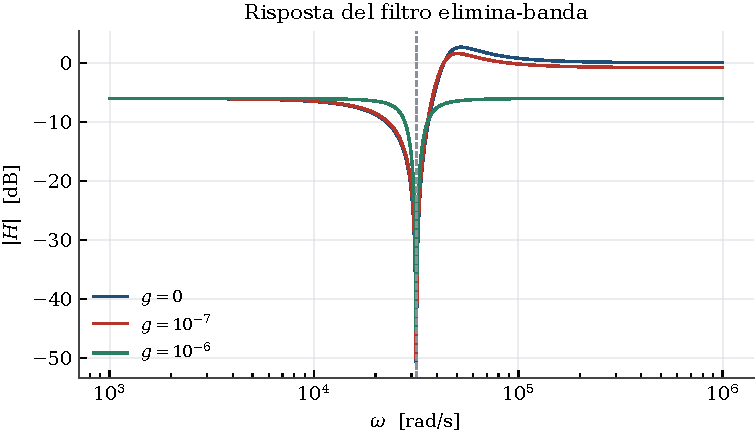
\includegraphics[width=0.86\linewidth]{../figures/notch_bode.pdf}
  \caption{Modulo della trasferenza della riga $\#4$ per tre valori della capacità aggiuntiva $G$. La tacca è alla pulsazione $\omega_n=1/\sqrt{LC}$ e non si sposta al variare del carico, mentre la profondità e la larghezza dipendono dai poli.}
  \label{fig:notch_bode}
\end{figure}

La forma è
\[
  H(s)=a\;\frac{s^2+\omega_n^2}{s^2+\dfrac{\omega_0}{Q}\,s+\omega_0^2},
\]
e le ultime quattro righe ne identificano i parametri:
\begin{itemize}[leftmargin=1.4em,itemsep=1pt]
  \item il guadagno in alta frequenza $a=\dfrac{C}{C+G}$, cioè il partitore capacitivo puro;
  \item la pulsazione del notch $\omega_n=\dfrac{1}{\sqrt{LC}}$, dove la trasferenza si annulla;
  \item la pulsazione dei poli $\omega_0=\dfrac{1}{\sqrt{\frac{LF}{L+F}\,(C+G)}}$, che coinvolge il parallelo delle due induttanze e la somma delle due capacità;
  \item il fattore di merito $Q=R(C+G)\,\omega_0$, che governa quanto stretta sia la banda soppressa.
\end{itemize}
È la forma in cui un filtro si progetta davvero: si sceglie $\omega_n$ in base alla frequenza da eliminare, e poi $Q$ in base a quanto stretta debba essere la tacca.

\section*{In sintesi}
\addcontentsline{toc}{section}{In sintesi}

Venti righe che portano un circuito dalla topologia alla forma canonica, con i controlli ai casi limite fatti per bene. È il quaderno meno speculativo della raccolta e l'unico che risponde a una domanda pratica; il fatto che stia nella stessa cartella insieme alle delta complesse e ai fattoriali semi-interi dice qualcosa su come venissero usati questi file.

